\chapter{Copula}
\label{ch-copula}

A copula in architecture is a domed roof. Here we will discuss a copula in Statistics.
It is probably called that in Statistics
because its probability density resembles a dome when its domain is 
the real plane $\RR^2$.

Suppose you know the marginals $P(x_i)$ with $x_i\in \RR$, for
$i=1,2, \ldots n$ 
of a probability distribution $P(x_1, x_2, \ldots, x_n)$,
but you don't know $P(x_1, x_2, \ldots, x_n)$
itself. There are
infinitely many
possible $P(x_1, x_2, \ldots, x_n)$'s
with those marginals.
Informally
speaking,
a {\bf copula} is one of those
$P(x_1, x_2, \ldots, x_n)$, a smooth one.
The dimension $n$ of
the domain of the copula,
is referred to as the
{\bf copula dimension}.
See Figs. \ref{fig-copula1}
and \ref{fig-copula2}
for examples of 2-dimensional copulas.

\begin{figure}[!h]
\begin{floatrow}
 \ffigbox{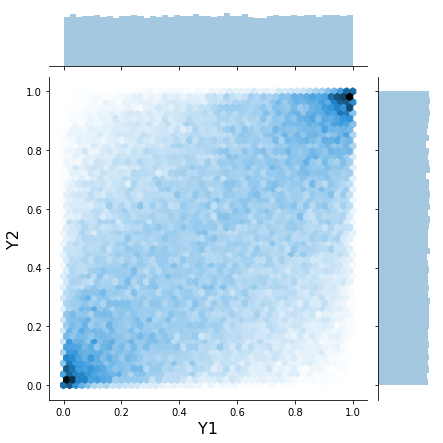
\includegraphics[width=2.5in]
 {copula/copula1.png}}
 {\caption{Example of 2-dimensional copula
 with uniform marginals}
 \label{fig-copula1}}
 \ffigbox{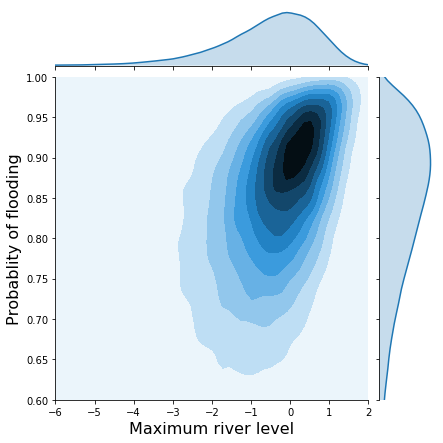
\includegraphics[width=2.5in]
 {copula/copula2.png}}
 {\caption{Example of 2-dimensional copula
 with skewed bell-shaped marginals.}
 \label{fig-copula2}}
\end{floatrow}
\end{figure}





\begin{figure}[h!]
$$
\xymatrix{
\rvu_1\ar[dd]
&\rvx_1\ar[l]_{\Phi_{\rvx_1}}\quad P(x_1)
\\
\\
\rvu_2
&\rvx_2\ar[l]_{\Phi_{\rvx_2}}\quad P(x_2)
}
\xymatrix{\\=P(u^2, x^2)=}
\xymatrix{
\rvx_1\ar[dd]
&\rvu_1\ar[l]_{\Phi_{\rvx_1}^{-1}}\quad P(u_1)
\\
\\
\rvx_2
&\rvu_2\ar[l]_{\Phi_{\rvx_2}^{-1}}\quad P(u_2)
}
$$
\caption{Graphical representation
of Eq.(\ref{eq-copula-def}) for $n=2$.
$\Phi_{
\rvx_i}(x_i) = P(\rvx_i<x_i)$
is the cumuulative probability
distribution of $\rvx_i$,
and we define
$u_i = \Phi_{\rvx_i}(x_i)$}
\label{fig-copula-def-n-2}
\end{figure}

More precisely,
a copula in Statistics is 
defined as follows.
Let $u^n = [u_i]_{i=1}^n\in \RR^n$ and $x^n= [x_i]_{i=1}^n\in\RR^n$ be $n$ 
dimensional column vectors.
A
{\bf copula density}  is a probability density $P(u^n|x^n)$
such that (see Fig.\ref{fig-copula-def-n-2})

\beq
\underbrace{P(u^n|x^n)}_{\text{Choice of Copula}}
\underbrace{\prod_{i=1}^n 
\underbrace{P(x_i)}_{\text{arbitrary dist.}}
}_{\text{input marginals}}=
P(u^n, x^n)=
\underbrace{P(x^n|u^n)}_{\text{Output joint dist.}}
\underbrace{
\prod_{i=1}^n
\underbrace{ P(u_i)}_{
\text{Uniform over } [0,1]}
}_{=1}
\label{eq-copula-def}
\eeq
where, for all $i$, $P(u_i)=1$ is the uniform distribution 
over the interval $u_i\in[0,1]$.



A {\bf copula} $C(u^n|x^n)$ is defined as the  
cumulative probability distribution
of its copula density.

\beqa
C(u^n|x^n) &=& \prod_{i=1}^n
\left\{
\int_{-\infty}^{u_i}du_i'
\right\}P(\rvu^n=(u')^n|x^n)
\\
&=&
P(\rvu_1<u_1, \rvu_2<u_2, \ldots, \rvu_n<u_n)
\eeqa

\beq
\partial_{u_1}
\partial_{u_2}
\ldots \partial_{u_n}
C(u^n|x^n) = P(u^n|x^n)
\eeq

A copula can be defined
without allusion
to its density,
as a  map $C:[0,1]^n\rarrow [0,1]$
that is a cumulative probabilty distribution
 with uniform marginals.
There are copulas
that are well-defined but
not differentiable, so, 
technically, without smoothing,
their 
copula density does not exist.







\hrule
We achieve a uniform distribution
for each $u_i$ by setting

\beqa
\rvu_i &=&\int_{-\infty}^{\rvx_i}dx'_i\;
 P(\rvx_i=x'_i) 
 \\
 &=& \left[P(\rvx_i< x_i)\right]_{x_i\rarrow
 \rvx_i}
 \label{eq-u-i-is-one}
\eeqa
for each $i=1,2, \dots, n$.
Note that 
this does NOT imply that the 
$\{\rvu_i|\forall i\}$ are mutually
independent; that would only
be true if the $\{\rvx_i|\forall i\}$
were mutually independent,
which is generally not true.
It does imply the following:

\begin{claim} Eq.(\ref{eq-u-i-is-one})
implies that the marginal
$P(u_i)=1$ is a uniform distribution on $[0,1]$.
\end{claim}
\proof

For $0<\eps<<1$,
\beq
\rvu_i = P(\rvx_i<\rvx_i+\eps)=1
\eeq
If that doesn't convince you, here is another 
proof.
Define

\beq
\Phi_{\rvx_i}(x_i) = P(\rvx_i<x_i)
\eeq
Then
\beqa
P(\rvu_i<u_i)
&=&
P(\Phi_{\rvx_i}(\rvx_i)<u_i)
\\
&=&
P(\rvx_i<\Phi_{\rvx_i}^{-1}(u_i))
\\
&=&
\Phi_{\rvx_i}\left(
\Phi_{\rvx_i}^{-1}(u_i)
\right)
\\
&=&
u_i
\eeqa
Hence,

\beqa
P(\rvu_i=u_i)&=&
\pder{}{u_i}\int_{-\infty}^{u_i}
du'_i \; P(\rvu_i=u'_i)
\\
&=&
\pder{P(\rvu_i<u_i)}{u_i}
\\ &=& 1
\eeqa
\qed


